Let $(X, \M, \mu)$ and $(Y, \mathcal{N}, \nu)$ be measure spaces and let
\[
\A := \left\{ \bigcup_{i=1}^n A_i \times B_i \ : \ A_i \in \M, B_i \in \mathcal{N}, \text{ and } (A_i \times B_i) \cap (A_j \times B_j) = \o \text{ if } i \neq j \right\}.
\]
\begin{enumerate}
\item Prove that $\A$ is an algebra.
\begin{pf}
	Consider $\{ R_i \}_{i=1}^k \subset \A$. Then, for all $1 \leq i \leq k$, $R_i =  \bigcup_{i=1}^n A_i \times B_i \ : \ A_i \in \M, B_i \in \mathcal{N}, \text{ and } (A_i \times B_i) \cap (A_j \times B_j) = \o \text{ if } i \neq j$. We will show $\bigcup_{i=1}^k R_i  \in \A$ inductively. Notice 
	\[
	R_i \cup R_j=\bigcup_{i=1}^n A_i \times B_i \cup \bigcup_{j=1}^m C_j \times D_j=\bigcup_{i=1}^n  \bigcup_{j=1}^m (A_i \times B_i \cup C_j \times D_j)
	\] So, we will first consider the union of two rectangles, $A \times B$ and $C \times D$ and write $(A \times B) \cup (C \times D)$ as the union of disjoint rectangles: \\.
	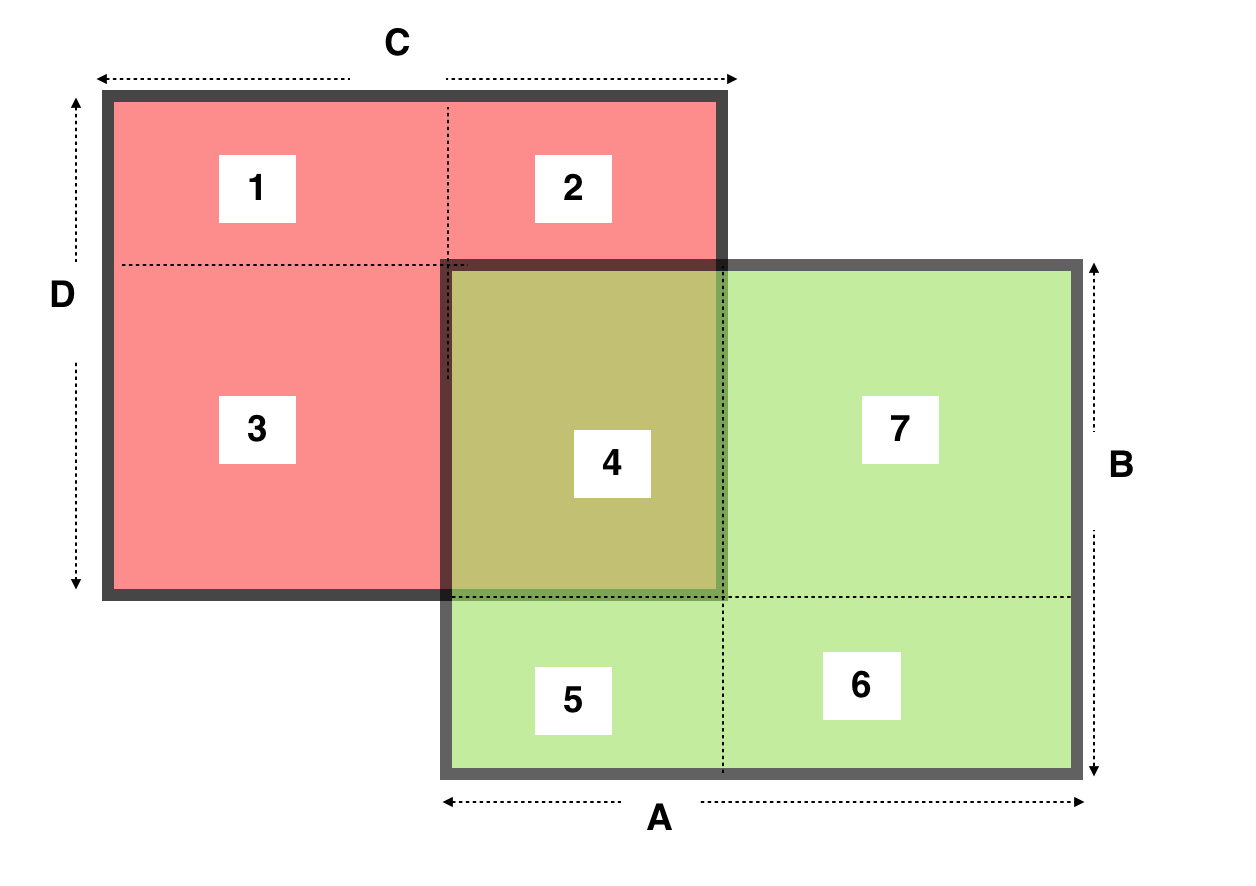
\includegraphics[scale=.45]{oct2pic.png}\\ 
\[
\text{Notice we can write  } (A \times B) \cup (C \times D) \text{ as the union of the disjoint rectangles, labeled 1 to 7 in the figure above.}  
\]
\[
(A \times B) \cup (C \times D) =((A\backslash C) \times (B \backslash D)) \ \cup \ ((A\backslash C^c) \times (B \backslash D)) \ \cup \ ((A\backslash C) \times (B \backslash D^c)) \ \cup \ ((A\backslash C^c) \times (B \backslash D^c)) \ \cup 
\]
\[
((A\backslash C^c) \times (D \backslash B)) \ \cup \ ((C\backslash A) \times (D \backslash B)) \ \cup \ \ ((C\backslash A) \times (B \backslash D^c)) 
\]
From the figure, we can see that all these rectangles are disjoint; thus, $R_i \cup R_j \in \A$.\\ Assume that $\bigcup_{i=1}^{n}R_i \in \A$. Then,  $\bigcup_{i=1}^{n}R_i \cup R_j= \bigcup_{i=1}^n (R_i \cup R_j)$. Our previous conclusion implies that $(R_i \cup R_j) \in \A$. So, since $\bigcup_{i=1}^{n}R_i \in \A$ and $(R_i \cup R_j) \in \A$, $\bigcup_{i=1}^{n+1} (R_i) \in \A$. Thus, $\bigcup_{i=1}^k R_i  \in \A$. \\
Next, to show $R_i^c \in \A$ for any $i$, consider $(A \times B) \cap (C \times D)$ in the figure. Notice $(A \times B) \cap (C \times D)=(A \cap C) \times (B \cap D) \in \A$. Thus, inductively, we can show $\bigcap_{i=1}^n R_i \in \A$. So, by inspection of figure, we can see
\[
R_i^c=\left(\bigcup_{i=1}^n A_i\times B_i \right)^c=\bigcap_{i=1}^n (A_i\times B_i)^c=\bigcap_{i=1}^n\left( (A_i^c\times B_i^c) \cup (A_i\times B_i^c) \cup (A_i^c\times B_i)\right). 
\]
Notice $(A_i^c\times B_i^c), (A_i\times B_i^c), (A_i^c\times B_i)$ are disjoint so $(A_i^c\times B_i^c) \cup (A_i\times B_i^c) \cup (A_i^c\times B_i) \in \A$. Thus, $\bigcap_{i=1}^n\left( (A_i^c\times B_i^c) \cup (A_i\times B_i^c) \cup (A_i^c\times B_i)\right) \in \A$, so $R_i^c \in \A$ for any $i$.\\
Hence, $\A$ is an algebra. 
\end{pf}

\item Prove that if $\mu$ and $\nu$ are $\sigma$-finite then so is $\mu \times \nu$. 
\begin{pf}
	Assume $\mu$ and $\nu$ are $\sigma$-finite. Then, $X=\bigcup_{j=1}^\infty A_j$ with $\mu(A_j)<\infty$ for all $j$ and $Y=\bigcup_{i=1}^\infty B_i$ with $\nu(B_i)< \infty$ for all $i$. Then, $X \times Y=\bigcup_{j=1}^\infty A_j \times \bigcup_{i=1}^\infty B_i=\bigcup_{j=1}^\infty \bigcup_{i=1}^\infty A_j \times B_i$. Since $\mu(A_j)<\infty$ and $\nu(B_i)< \infty$ for all $i, j$, $\mu(A_j)\nu(B_i)<\infty$ for all $i, j$. Therefore, $\mu \times \nu$ is $\sigma$-finte.
\end{pf}
\end{enumerate}
